\documentclass[a4paper, 12pt]{article}
\usepackage{deuresutils}
\usepackage{graphicx}
\graphicspath{ {images/} }

\title{Lliurament 3}
\asignatura{Càlcul en Diverses Variables}
\author{Eduardo Pérez Motato}
\niu{NIU: 1709992}
\date{27/05/2024}

\begin{document}
    \makeheader

    \setcounter{numex}{56}
    \begin{exercici}
        Sigui $f\left(x,y,z\right) = y^3 + xz^2$. Determineu el màxim i el mínim absolut de $f$
        sobre la superfície de l'esfera centrada a l'origen i de radi $1$.
    \end{exercici}
    \begin{solucio}
        Per aixó hem de fer servir el teorema dels multiplicadors de Lagrange.\\
        Definim $g(x,y,z) := x^2+y^2+z^2-1$, ara si fem $\nabla(f-\lambda g)(x_0) = 0$ llavors $x_0$
        és un extrem relatiu condicionat a la superfície. Ara, calqulem:
        \begin{displaymath}
            \begin{split}
                (0,0,0) &=\nabla(f-\lambda g)(x_0)\\
                  &=\nabla\left(y^3+xz^2 - \lambda(x^2+y^2+z^2-1)\right)(x_0)\\
                  &=\left(z^2 - \lambda(2x), 3y^2 - \lambda(2y), 2xz - \lambda(z^2)\right)(x_0)
            \end{split}
        \end{displaymath}
        Llavors
        \begin{displaymath}
            \begin{cases}
                z^2 - \lambda(2x) = 0\\
                3y^2 - \lambda(2y) = 0\\
                2xz - \lambda(z^2) = 0\\
                x^2+y^2+z^2 = 1
            \end{cases}
        \end{displaymath}
        Llavors sabem que $y = 0$ o $y = \frac{2\lambda}{3}$. També arribem a què $x = \frac{z^2}{2\lambda}$ i 
        llavors $\frac{z^3-\lambda z^2}{\lambda} = 0$. Per alló tenim els seguents casos:
        \begin{displaymath}
            \begin{cases}
                z = 0 \Rightarrow x = 0\text{, fent que } y = 1\\
                z = \lambda \Rightarrow x = \frac{\lambda}{2}\text{, aixó no restringeix }y\text{ que pot ser els dos}.
            \end{cases}
        \end{displaymath}
        En el segon, calculem $\lambda$ en ambdos casos: $y = 0, y = \frac{2\lambda}{3}$.\\
        En el primer, $\left(\frac{\lambda}{2}\right)^2+\lambda^2 = 1$, llavors $\lambda = \pm\frac{2\sqrt{5}}{5}$\\
        En el segon, $\left(\frac{\lambda}{2}\right)^2+\left(\frac{2\lambda}{3}\right)^2+\lambda^2 = 1$,
        llavors $\lambda = \pm\frac{6\sqrt{61}}{61}$\\\\
        Finalment, tenim els seguents punts:
        \begin{enumerate}
            \item $x_1 = \left(0, 1, 0\right) \Rightarrow f(x_1) = 1$
            \item $x_2 = \left(\frac{\sqrt{5}}{5}, 0, \frac{2\sqrt{5}}{5}\right) \Rightarrow f(x_2) = \frac{4\sqrt{5}}{25}$
            \item $x_3 = \left(\frac{3\sqrt{61}}{61}, \frac{4\sqrt{61}}{61}, \frac{6\sqrt{61}}{61}\right) \Rightarrow f(x_3) = \frac{172\sqrt{61}}{3721}$
            \item $x_4 = \left(-\frac{\sqrt{5}}{5}, 0, -\frac{2\sqrt{5}}{5}\right) \Rightarrow f(x_4) = -\frac{4\sqrt{5}}{25}$
            \item $x_5 = \left(-\frac{3\sqrt{61}}{61}, -\frac{4\sqrt{61}}{61}, -\frac{6\sqrt{61}}{61}\right) \Rightarrow f(x_5) = -\frac{172\sqrt{61}}{3721}$
        \end{enumerate}
        D'aquests, el minim absolut és $x_5$ i el maxim absolut $x_1$.
    \end{solucio}

    \setcounter{numex}{58}
    \begin{exercici}
        Sigui $D$ el disc tancat centrat a l'origen i de radi $1$ i sigui $f\left(x,y\right) = x^2+xy+y^2$.
        Justifiqueu per què $f$ té màxim i mínim absoluts sobre $D$ i trobeu-los.
    \end{exercici}
    \begin{solucio}
        $D = \left\{\left(x,y\right)\in\mathbb{R}^2: x^2+y^2 \leq 1\right\}$. Llavors, els máxims i
        minims absoluts d'un compacte com $D$ es poden calcular gràcies a $g(x,y) := x^2+y^2-1$.
        Llavors, en aplicar el teorema dels multiplicadors de Lagrange tindrem el següent
        \begin{displaymath}
            \begin{split}
                0 &= \nabla\left(x^2+xy+y^2 - \lambda \left(x^2+y^2-1\right)\right)\\
                &= \nabla\left((x^2+y^2)(1-\lambda)+xy-\lambda\right)\\
                &= \left(2x(1-\lambda)+y, 2y(1-\lambda)+x\right)
            \end{split}
        \end{displaymath}
        Aixó gènera les seguents equacions:
        \begin{displaymath}
            \begin{cases}
                2x(1-\lambda)+y = 0\\
                x+2y(1-\lambda) = 0\\
                x^2+y^2 = 1
            \end{cases}
        \end{displaymath}
        Podem veure que $x = -2y(1-\lambda)$, de alli treiem que $0 = (-4(1-\lambda)^2+1)y$.\\
        Si $y = 0$, $x = 0$. Aixó no compleix la tercera equació. En canvi, si fem $(-4(1-\lambda)^2-1) = 0 \Rightarrow \lambda = \pm \frac{1}{2}$.
        Aixó fa que $x = \pm y$.\\
        Si fem aixó, $2x^2 = 1 \Rightarrow x = \pm\frac{\sqrt{2}}{2}$. Finalment, tenim aquests
        quatre punts
        \begin{enumerate}
            \item $x_1 = \left(\frac{\sqrt{2}}{2}, \frac{\sqrt{2}}{2}\right) \Rightarrow f(x_1) = 3.$
            \item $x_2 = \left(\frac{\sqrt{2}}{2}, -\frac{\sqrt{2}}{2}\right) \Rightarrow f(x_2) = 1.$
            \item $x_3 = \left(-\frac{\sqrt{2}}{2}, \frac{\sqrt{2}}{2}\right) \Rightarrow f(x_3) = 1.$
            \item $x_4 = \left(-\frac{\sqrt{2}}{2}, -\frac{\sqrt{2}}{2}\right) \Rightarrow f(x_4) = 3.$
        \end{enumerate}
        Llavors, els extrems relatius són $x_1, x_2, x_3, x_4$.\\
        Ara hem de fer $\nabla\left(x^2+xy+y^2\right) = 0$. Llavors, $\left(2x+y, 2y+x\right) = \left(0, 0\right)$.\\
        L'unica solució d'aquesta equació és $\left(0,0\right)$, que si és evalua és $0$.\\
        El máxim absolut és $x_1$ i $x_3$ i el mínim és $\left(0,0\right)$
    \end{solucio}

    \begin{exercici}
        Feu el mateix si $D$ és el quadrat tancat de vértexs $\left(0,0\right),\left(1,0\right),\left(0,1\right),\left(1,1\right)$.
    \end{exercici}
    \begin{solucio}
        En aquest cas, sabem que $g_1(x) = 1$, $g_2(x) = 0$, $g_3(y) = 1$, $g_4(x) = 0$.\\
        Veiem que si fem $\nabla\left(f-\lambda g_n\right) = 0$ equival a $\nabla f = 0$. Evaluem
        els seguents punts:
        \begin{enumerate}
            \item $x_1 = \left(0, 0\right) \Rightarrow f(x_1) = 0.$
            \item $x_2 = \left(1, 0\right) \Rightarrow f(x_2) = 1.$
            \item $x_3 = \left(0, 1\right) \Rightarrow f(x_3) = 1.$
            \item $x_4 = \left(1, 1\right) \Rightarrow f(x_4) = 3.$
        \end{enumerate}
        Llavors, veiem clarament que el máxim és $\left(1,1\right)$ i el minim és $\left(0,0\right)$.
    \end{solucio}

    \setcounter{numex}{61}
    \begin{exercici}
        Trobeu els extrems absoluts de les funcions següents sobre els conjunts que us indiquen.
        \begin{itemize}
            \item[a)] $f\left(x,y\right) = x^2+y^2+2x$ sobre $\left\{\left(x,y\right): x^2+y^2\leq 1, y\geq x\right\}$
        \end{itemize}
    \end{exercici}
    \begin{solucio}
        Primer calcularem els extrems relatius de $f$:
        $\nabla f = 0 \Rightarrow \left(2x+2, 2y\right) \Rightarrow \left(-1, 0\right)$. Aquest punt
        està al domini.\\
        Ara, farem mitjançants els multiplicadors de Lagrange la resta de punts.\\
        \begin{displaymath}
            \begin{split}
                \left(0,0\right) &= \nabla\left(x^2+y^2+2x - \lambda\left(x^2+y^2-1\right)\right)\\
                &= \nabla\left(2x +\left(1 - \lambda\right)\left(x^2+y^2\right)-\lambda\right)\\
                &= \left(2 +\left(1 - \lambda\right)2x, 2y\left(1 - \lambda\right)\right)
            \end{split}
        \end{displaymath}
        Aixó ens deixen les seguents equacions
        \begin{displaymath}
            \begin{cases}
                0 = 2+2x\left(1 - \lambda\right)\\
                0 = 2y\left(1 - \lambda\right)\\
                1 = x^2+y^2
            \end{cases}
        \end{displaymath}
        Aixó fa que o $\lambda = 1$ o $y = 0$. La primera ens fa arribar a una contradicció, així
        que ha de ser la segona, fent que $x = \pm1$.\\
        $\left(1,0\right)$ no está al domini i $\left(-1, 0\right)$ ja l'hem anotat.\\
        Ara, fem el mateix procés amb $g(x,y) := x - y$.\\
        \begin{displaymath}
            \begin{split}
                \left(0,0\right) &= \nabla\left(x^2+y^2+2x - \lambda\left(x-y\right)\right)\\
                &= \nabla\left(x^2+y^2+2x - \lambda\left(x-y\right)\right)\\
                &= \nabla\left(2x+2 - \lambda, 2y + \lambda\right)
            \end{split}
        \end{displaymath}
        Aixó ens deixen aquestes equacions
        \begin{displaymath}
            \begin{cases}
                0 = 2x+2-\lambda\\
                0 = 2y+\lambda\\
                0 = x-y
            \end{cases}
        \end{displaymath}
        Veiem que $\lambda = -2y$ i $\lambda = 2x+2$, aixó fa que $2x+2+2y = 0$, el que fa que
        $x=-\frac{1}{2}$ i $y = -\frac{1}{2}$, aquests estan dintre del domini.
        Llavors, ara evaluem els seguents punts:
        \begin{enumerate}
            \item $x_1 = \left(-1, 0\right) \Rightarrow f(x_1) = -1$
            \item $x_2 = \left(-\frac{1}{2}, -\frac{1}{2}\right) \Rightarrow f(x_2) = -\frac{1}{2}$
            \item $x_3 = \left(\frac{\sqrt{2}}{2}, \frac{\sqrt{2}}{2}\right) \Rightarrow f(x_3) = 1+\sqrt{2}$
            \item $x_4 = \left(-\frac{\sqrt{2}}{2}, -\frac{\sqrt{2}}{2}\right) \Rightarrow f(x_4) = 1-\sqrt{2}$
        \end{enumerate}
        Aixó ens dona que $x_3$ és el máxim i $x_1$ és el minim. 
    \end{solucio}
    
    \setcounter{numex}{64}
    \begin{exercici}
        Calculeu les integrals següents intercanviant els límits d'integració i dibuixeu el domini
        sobre el qual esteu integrant.
        \begin{itemize}
            \item[c)] $$\int_{0}^{4}\int_{y/2}^{2} e^{x^2}dxdy$$
        \end{itemize}
    \end{exercici}
    \begin{solucio}
        La regió que aixó crea és un triangle amb vertex $\left(0,0\right), \left(0,4\right), \left(2,0\right)$, és dir:
        \begin{center}
            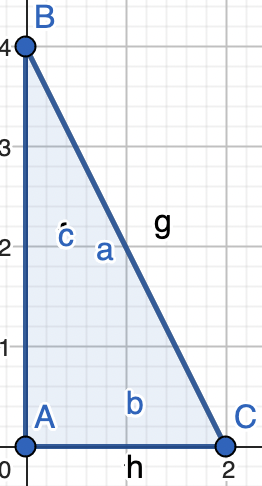
\includegraphics[width=0.125\textwidth]{1.png}\\
        \end{center}
        Intercanviant, tenim.
        $$\int_0^2\int_{2x}^4e^{x^2} dydx = \int_0^2 4e^{x^2}-2xe^{x^2} dx$$
        I aixó després de molta estona no he sabut calcular % Realment es que aquest intercanvi de variables és diferent el resultat lol
    \end{solucio}

    \setcounter{numex}{66}
    \begin{exercici}
        Escriviu $\iint_D fdxdy$ com a integral iterada i calculeu-la.
        \begin{itemize}
            \item[a)] $f\left(x,y\right)=\frac{y}{x^2+y^2}$ i $D$ és el triangle limitat per les
            rectes $y = x, y = 2x$ i $x = 2$.
            \item[b)] $f\left(x,y\right)=x$ i $D$ és el sector circular del primer quadrant limitat
            per la circunferència $x^2+y^2=25$ i les rectes $y=0$, $y = x$.
        \end{itemize}
    \end{exercici}
    \begin{solucio}
        \begin{itemize}
            \item[a)] $D = \left\{\left(x,y\right): x\leq y\leq2x\leq4\right\}$, llavors tenim $$\int_0^2\int_{x}^{2x}\frac{y}{x^2+y^2}dydx$$
            si aixó ho fem iterativament, primer hem de calcular $\int_{x}^{2x}\frac{y}{x^2+y^2}dy$,
            que és el seguent:
            $$\int_{x}^{2x}\frac{y}{x^2+y^2}dy = \frac{1}{2}\int_{x}^{2x}\frac{1}{x^2+t} dt = \frac{1}{2}\log(x^2+y^2)\bigg\rvert_{y=x}^{y=2x} = \frac{1}{2}\log{\frac{5x^2}{2x^2}} = \frac{1}{2}\log{\frac{5}{2}}$$
            i ara, tenim el seguent
            $$\int_0^2 \frac{1}{2}\log{\frac{5}{2}} dx = \frac{1}{2} \log{\frac{5}{2}} \int_0^2 1 dx = \frac{1}{2} \log{\frac{5}{2}} x\bigg\rvert_{x=0}^{x=2} = \log{\frac{5}{2}}$$
            i aquesta és la solució.
            \item[b)] $D = \left\{\left(x,y\right): x^2+y^2 \leq 25, x \geq y \geq 0\right\} = \left\{\left(r,\theta\right):r \leq 5, 0\leq\theta\leq\frac{\pi}{4}\right\}$, llavors
            $$\int_{0}^{5}\int_{0}^{\frac{\pi}{4}}r^2\cos{\theta}d\theta dr$$
            si aixó ho fem iterativament, primer hem de calcular $\int_{0}^{\frac{\pi}{4}}r^2\cos{\theta}d\theta$, que és el seguent:
            $$\int_{0}^{\frac{\pi}{4}}r^2\cos{\theta}d\theta = r^2\int_{0}^{\frac{\pi}{4}}\cos{\theta}d\theta = r^2\sin{\theta}\bigg\rvert_{\theta=0}^{\theta=\frac{\pi}{4}} = \frac{\sqrt{2}r^2}{2}$$
            i ara, tenim el seguent
            $$\int_{0}^{5} \frac{\sqrt{2}r^2}{2} dr = \frac{\sqrt{2}}{2} \int_{0}^{5} r^2 dr = \frac{\sqrt{2}}{2} \frac{r^3}{3}\bigg\rvert_0^5 = \frac{125\sqrt{2}}{6}$$
            i aquesta és la solució.
        \end{itemize}
    \end{solucio}


    \setcounter{numex}{77}
    \begin{exercici}
        Calculeu el centre de masses de $\left\{\left(x,y\right): 1\leq x^2+y^2 \leq 4, x\geq0, y \geq 0\right\}$, si la densitat de massa ve donada per $\rho\left(x,y\right) = x^2+y^2$.
    \end{exercici}
    
    \begin{solucio}
        $x_{cm} = \iint_\Omega x\rho\left(x,y\right)dxdy$, analogament amb $y_{cm}$.\\
        $\Omega = \left\{\left(r, \theta\right): 1\leq r \leq 2, 0 \leq \theta \frac{\pi}{2}\right\}$\\
        Llavors, tenim:
        $$x_{cm} = \int_{1}^{2}\int_{0}^{\frac{\pi}{2}} r^4\cos{\theta}d\theta dr = \int_{1}^{2} r^4 dr = \frac{31}{5}$$
        $$y_{cm} = \int_{1}^{2}\int_{0}^{\frac{\pi}{2}} r^4\sin{\theta}d\theta dr = \int_{1}^{2} r^4 dr = \frac{31}{5}$$

    \end{solucio}

    \begin{exercici}
        Poseu els límits d'integració si feu servir coordenades cilíndriques per integrar una funció
        sobre les regions que us indiquen.
        \begin{itemize}
            \item[b)] $B = \left\{\left(x,y,z\right)\in\mathbb{R}^3 : z^2\leq x^2+y^2\leq z\right\}$
        \end{itemize}
    \end{exercici}

    \begin{solucio}
        $B = \left\{\left(r, \theta, z\right): z^2 \leq r^2 \leq z\right\}$
        $$\int_{0}^{2\pi}\int_{0}^{1}\int_{z^2}^{z} f(r\cos{\theta}, r\sin{\theta}, z)r dr dz d\theta$$
    \end{solucio}
    
    \begin{exercici}
        Calculeu, fent servir coordenades cilíndriques, la integral de la funció $f\left(x,y,z\right) = xz$ sobre les regions de l'exercici anterior.
        \begin{itemize}
            \item[b)] $B = \left\{\left(x,y,z\right)\in\mathbb{R}^3 : z^2\leq x^2+y^2\leq z\right\}$
        \end{itemize}
    \end{exercici}

    \begin{solucio}
        $$\int_{0}^{2\pi}\int_{0}^{1}\int_{z^2}^{z} zr^2\cos{\theta} dr dz d\theta = \int_{0}^{2\pi}\int_{0}^{1} \cos{\theta} \frac{z^7-z^4}{3} dz d\theta = \int_{0}^{2\pi} \cos{\theta} \frac{3}{120} d\theta = 0$$
    \end{solucio}

    \setcounter{numex}{82}
    \begin{exercici}
        Calculeu les integrals següents.
        \begin{itemize}
            \item[b)] $$\iiint_\Omega (z^2+\sqrt{x^2+y^2}) dxdydz$$, on $\Omega = \left\{\left(x,y,z\right) \in \mathbb{R}^3 : y \leq 0, z^2\leq(x^2+y^2)\leq 2z\right\}$.
        \end{itemize}
    \end{exercici}

    \begin{solucio}
        Aquesta integral és més fácil si es fa un canvi de variable a coordenades cilindriques $\Omega = \left\{\left(r,\theta,z\right): 0 \leq \theta \leq \pi, z^2 \leq r^2 \leq 2z\right\}$,
        llavors l'integral és
        \begin{displaymath}
            \begin{split}
                \int_{0}^{\frac{1}{2}}\int_{z^2}^{2z}\int_{0}^{\pi}(z^2 + r)r d\theta drdz &= \int_{0}^{\frac{1}{2}}\int_{z^2}^{2z}\pi(z^2 + r)r drdz\\
                &= \int_{0}^{\frac{1}{2}}\int_{z^2}^{2z}z^2r\pi + r^2\pi drdz\\
                &= \int_{0}^{\frac{1}{2}}\frac{12z^4+16z^3-5z^6}{6}\pi dz\\
                &= \left(\frac{1}{80}+\frac{1}{24}-\frac{5}{5376}\right)\pi\\
                &= \frac{477\pi}{8960}
            \end{split}
        \end{displaymath}
    \end{solucio}

    \begin{exercici}
        Calculeu les integrals següents.
        \begin{itemize}
            \item[b)] $$\iiint_\Omega \frac{x}{\sqrt{x^2+y^2+z^2}} dxdydz$$, on $\Omega = \left\{\left(x,y,z\right) \in \mathbb{R}^3 : 1 \leq x^2+y^2+z^2\leq2, x \geq 0, y \geq 0, z \geq 0\right\}$.
        \end{itemize}
    \end{exercici}

    \begin{solucio}
        Aquesta integral és més fácil si pasem a coordenades esferiques tal que $\Omega = \left\{\left(\rho, \phi, \theta\right): 1 \leq \rho \leq \sqrt{2}, 0 \leq \phi \leq \frac{\pi}{2}, 0 \leq \theta \leq \frac{\pi}{2}\right\}$.
        Llavors, l'integral queda així
        $$\int_{1}^{\sqrt{2}} \int_{0}^{\frac{\pi}{2}} \int_{0}^{\frac{\pi}{2}}  \frac{\rho\sin{\phi}\cos{\theta}}{\rho}\rho^2\sin{\phi} d\phi d\theta d\rho$$
        Llavors, calculem
        \begin{displaymath}
            \begin{split}
                \int_{1}^{\sqrt{2}} \int_{0}^{\frac{\pi}{2}} \int_{0}^{\frac{\pi}{2}}  \rho^2\sin^2{\phi}\cos{\theta} d\phi d\theta d\rho &= \int_{1}^{\sqrt{2}} \int_{0}^{\frac{\pi}{2}} \rho^2\cos{\theta} \int_{0}^{\frac{\pi}{2}} \sin^2{\phi} d\phi d\theta d\rho\\
                &= \int_{1}^{\sqrt{2}} \int_{0}^{\frac{\pi}{2}} \frac{\pi}{4} \rho^2\cos{\theta} d\theta d\rho\\
                &= \int_{1}^{\sqrt{2}} \frac{\pi}{4} \rho^2 \int_{0}^{\frac{\pi}{2}} \cos{\theta} d\theta d\rho\\
                &= \int_{1}^{\sqrt{2}} \frac{\pi}{4} \rho^2 d\rho\\
                &= \frac{\pi}{4} \left(\frac{\rho^3}{3}\bigg\rvert_{1}^{\sqrt{2}}\right)\\
                &= \frac{2\sqrt{2}-1}{12}\pi\\
            \end{split}
        \end{displaymath}
    \end{solucio}
\end{document}